\documentclass[10pt,a4paper,twocolumn]{article}

\usepackage[T1]{fontenc} % extended font encoding
\usepackage{enumerate} % lists
\renewcommand{\familydefault}{\sfdefault} % sans-serif
\usepackage{microtype} % better text justification
\usepackage{graphicx} % allow including pictures
\usepackage{color} % colors for pictures
\usepackage{fancyhdr} % headers and footers
\usepackage{titling} % picture in the title
\usepackage{hyperref} % clickable links
\usepackage[left=2cm,right=2cm,top=3cm,bottom=3cm]{geometry} % wider and taller page

\pagenumbering{gobble} % hide page numbers
\setlength{\columnsep}{1cm} % space between columns
\setlength{\parskip}{\baselineskip} % paragraphs divided by empty lines
\setlength{\parindent}{0pt}

\pdfinfo{
   /Author (Zlosynth Instruments)
   /Title  (Kaseta - Build Manual)
}

% TODO: Bring this back. It is commented out to fix syntax highlighting
% \pretitle{%
%   \begin{center}
%   \Huge
% }
% \posttitle{%
%   \\
%   \vspace{2cm}
%   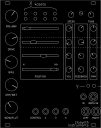
\includegraphics[width=16cm]{schema.pdf}
%   \end{center}
% }

\begin{document}

\title{Kaseta -- Build Manual}
\author{}
\date{}

\maketitle

\section{Overview}

You can always find the latest version of this build manual on
\url{https://zlosynth.com/kaseta-build-manual.pdf}.

This kit contains a printed circuit board (PCB) with all the surface mount
device (SMD) parts already pre-soldered. The through-hole components are left to
be assembled by you.

Pay attention to the orientation and position of all the parts. Desoldering them
would be difficult and may break the module. Also, be careful not to touch the
pre-soldered SMD parts with the soldering iron. Read through the whole manual
first. Make sure you understand all the steps before you start soldering.

\newpage

\section{Tools required}

\begin{itemize}
  \item Soldering iron
  \item Masking tape
  \item Flat head screwdriver
  \item Phillips head screwdriver
  \item Side-cutters
\end{itemize}

\newpage

\section{Bill of materials}

Start by unpacking all baggies into a bowl so you don't lose any components.

\begin{tabular}{@{}rl@{}}
  1 \texttimes & Front panel \\
  1 \texttimes & PCB (the black board) \\
  1 \texttimes & Daisy Patch Submodule (the yellow board) \\
  4 \texttimes & Green D-shaped pot without detent \\
  1 \texttimes & Green D-shaped pot with center detent \\
  5 \texttimes & M7 nut and washer \\
  5 \texttimes & Knob \\
  4 \texttimes & Slider potentiometer and cap \\
  9 \texttimes & Blue trim pot without detent \\
  5 \texttimes & Blue trim pot with center detent \\
  8 \texttimes & 3.5mm jack socket, M6 nut and washer \\
  1 \texttimes & Tactile button \\
  9 \texttimes & Red LED \\
  1 \texttimes & Male connector 2\texttimes5 \\
  4 \texttimes & Female connector 2\texttimes5 \\
  1 \texttimes & M2 flat screw \\
  1 \texttimes & M2 phillips screw \\
  1 \texttimes & M2 standoff \\
\end{tabular}

\section{Power and I2C}

Start by soldering the power and I2C connectors.

\begin{enumerate}
  \item Take the male 2\texttimes5 connector and put the side with shorter legs
    through the footprint marked as ``Power''. Make sure to put it on the
    correct side of the PCB.
  \item Solder a single pin in and check that the connector is upright. If it
    is not, heat up the pin and align the connector by pushing it against the
    board.
  \item Solder all the pins in.
\end{enumerate}

Repeat the process for the male 1\texttimes3 connector, placed in the ``I2C''
footprint.

\section{Daisy Patch Submodule}

The Daisy Patch Submodule is connected to the main PCB through a set of
connectors.

\begin{enumerate}
  \item Mount the four female 2\texttimes5 connectors on the pins of the Daisy
    Patch Submodule. See figure \ref{daisy}. This makes it easier to
    align all the connectors properly.
  \item Plug the connectors of the submodule into the black PCB through
    footprints marked as ``SM''. Make sure to put them on the correct side
    of the PCB, where all four connectors are marked.
  \item Solder all the pins in.
  \item Once done, carefully detach Daisy Patch Submodule to prevent it
    from getting damaged while progressing with the build. It may be a
    little difficult. Pull each connector by a millimeter at a time.
    The result is illustrated in figure \ref{connectors}.
\end{enumerate}

\begin{figure}[h]
  \centering
  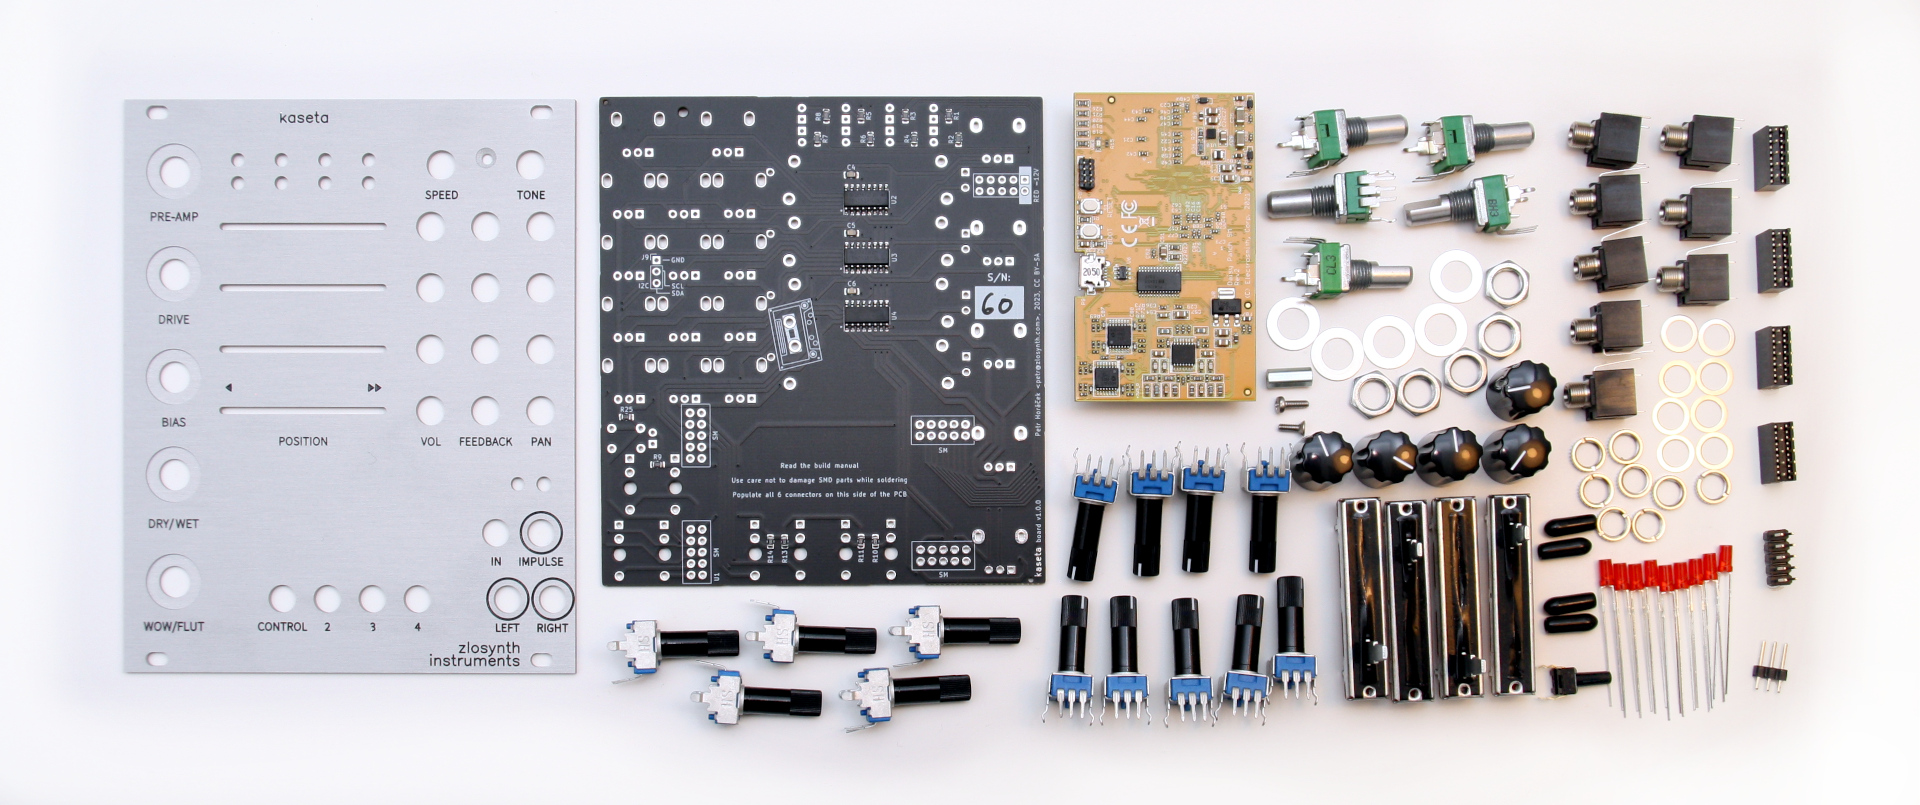
\includegraphics[width=\linewidth]{p01.jpg}
  \caption{All the components laid out}
\end{figure}

\begin{figure}[h]
  \centering
  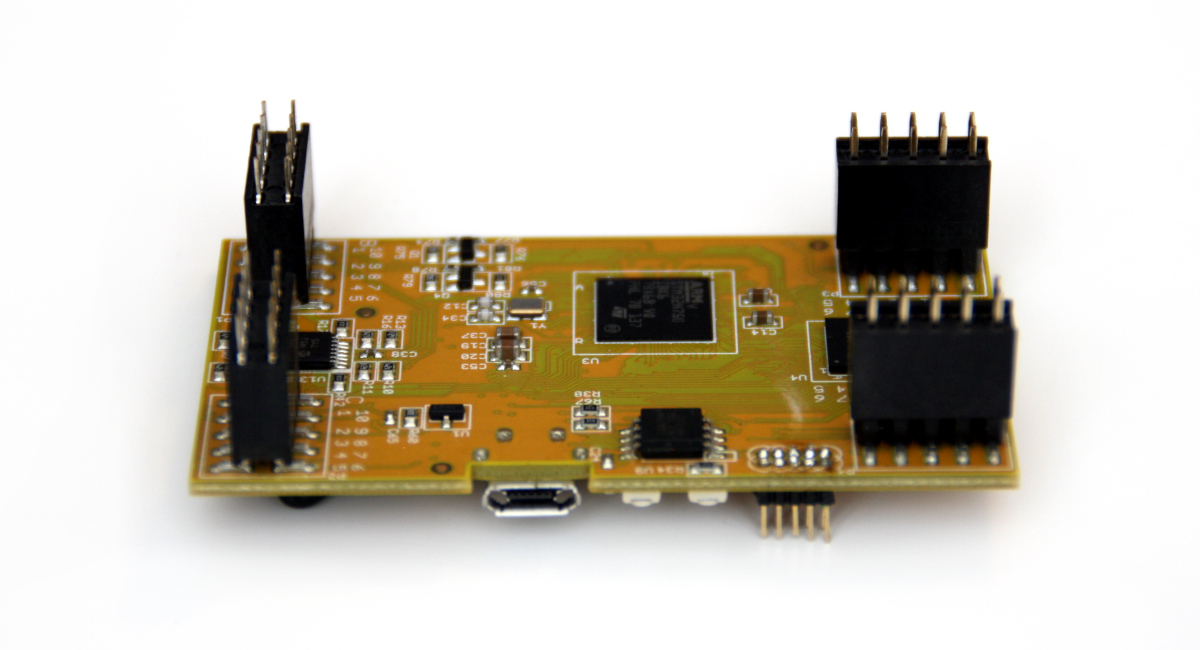
\includegraphics[width=\linewidth]{p02.jpg}
  \caption{Connectors mounted on the submodule}
  \label{daisy}
\end{figure}

\begin{figure}[h]
  \centering
  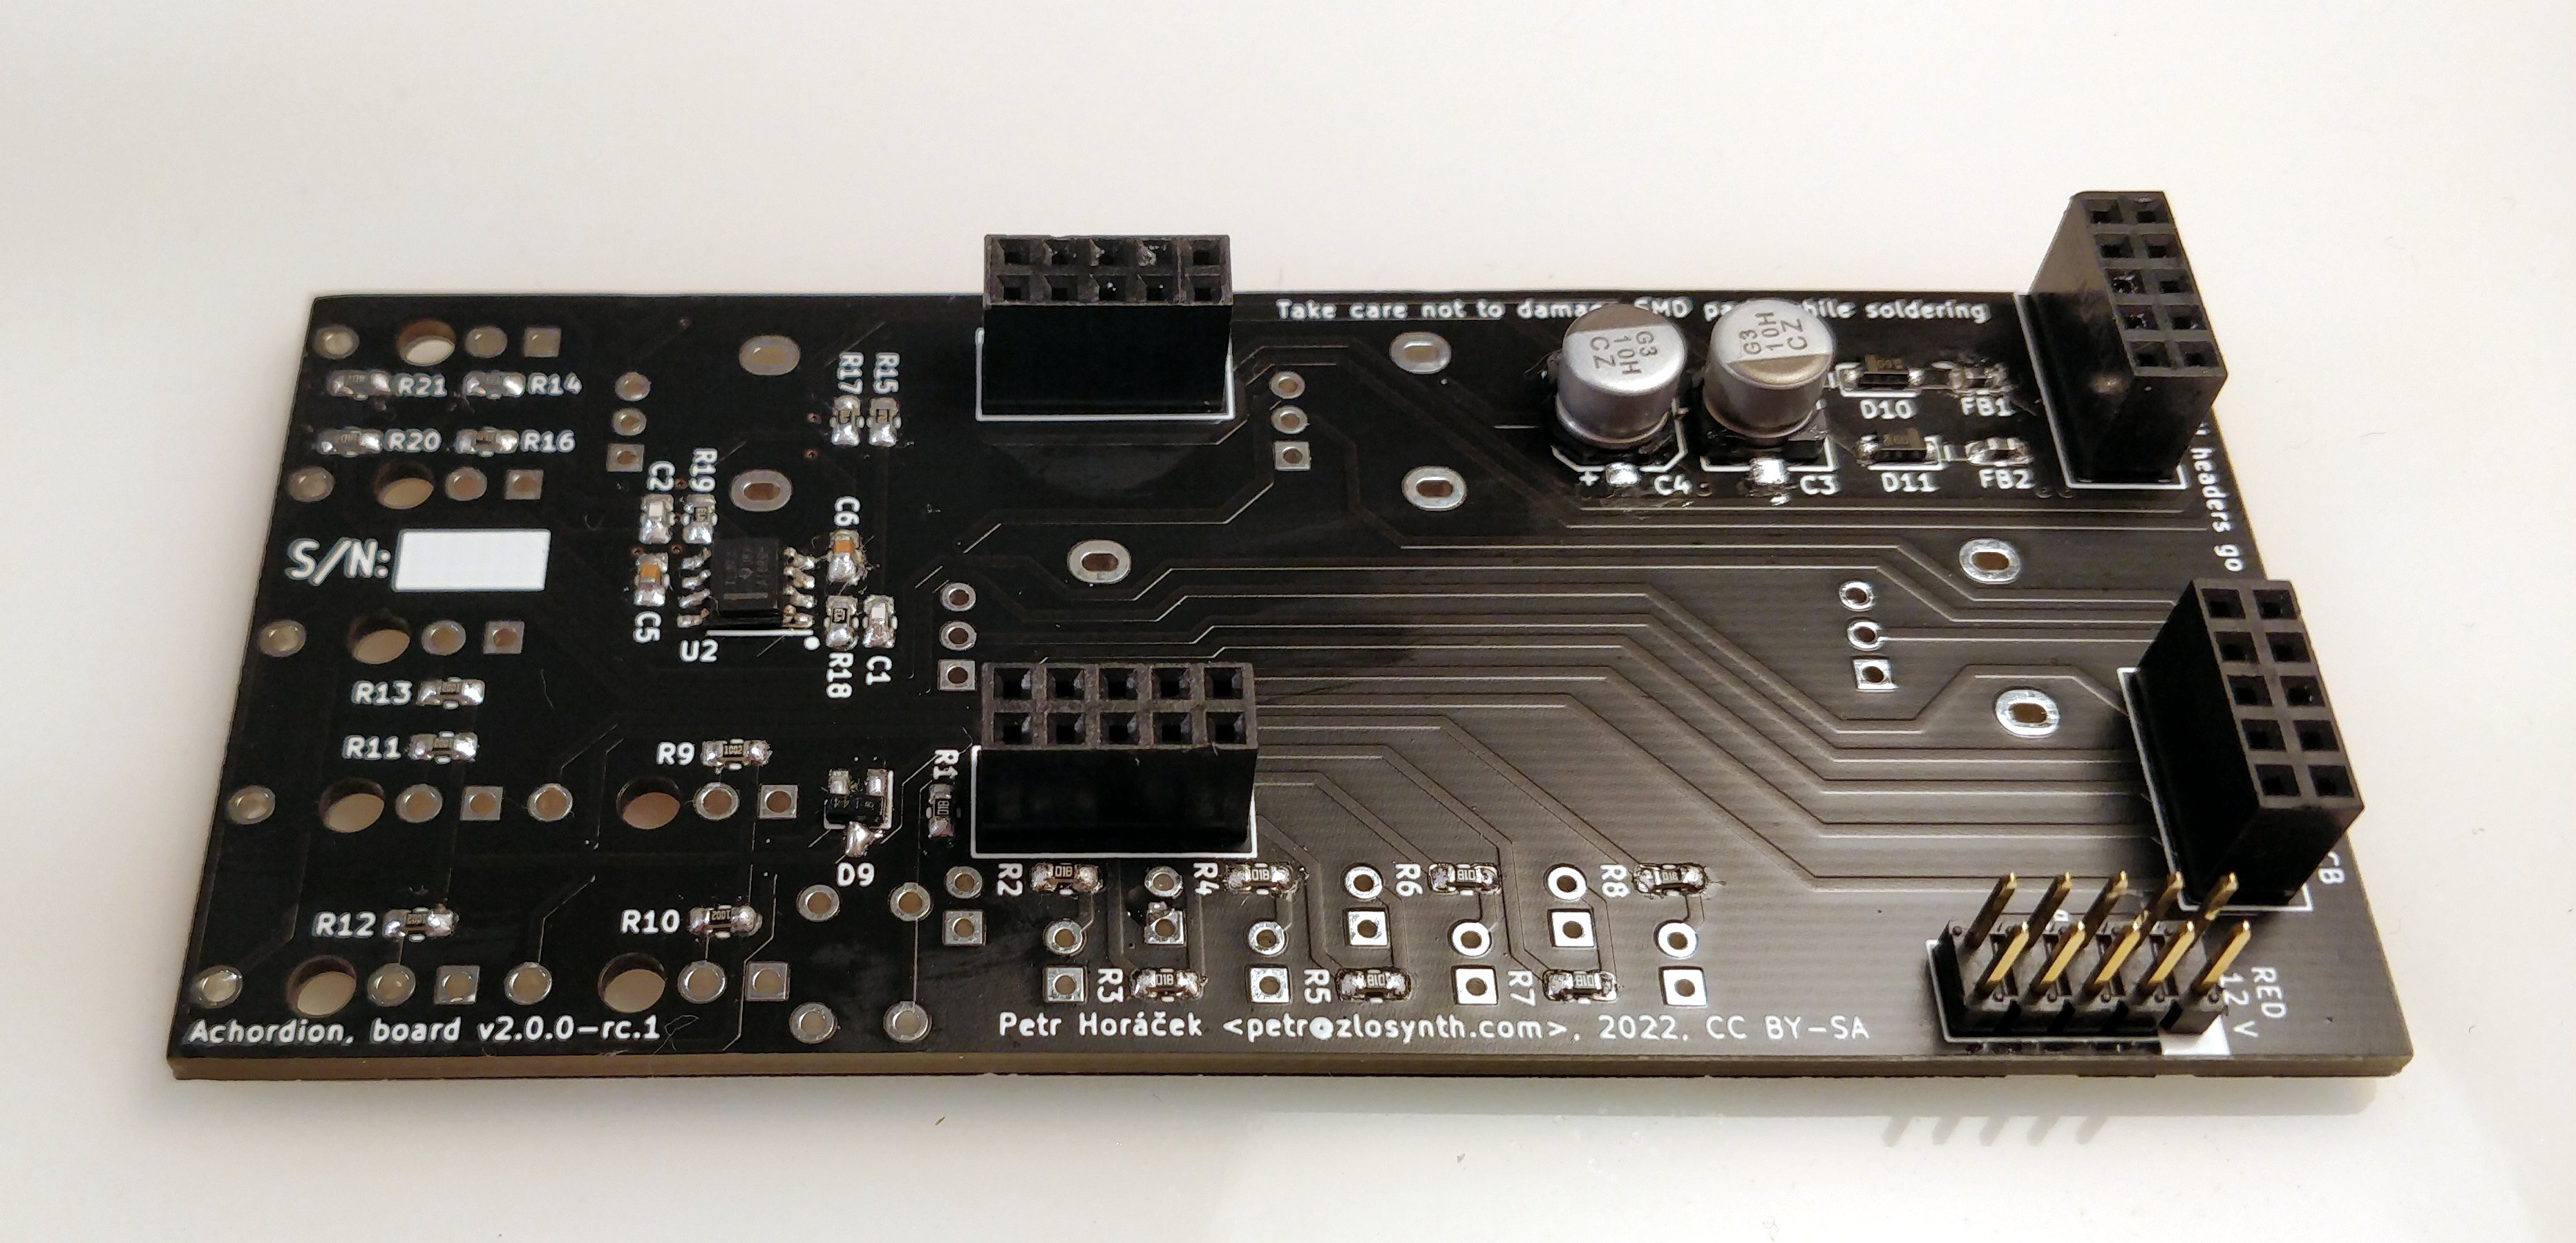
\includegraphics[width=\linewidth]{p03.jpg}
  \caption{The power and submodule connectors}
  \label{connectors}
\end{figure}

\clearpage

\section{Front panel}

Now when all the internal parts are soldered, the next step would be to assemble parts sitting in the front panel.

\begin{enumerate}
  \item Snap in the button. Take care not to bend its leg. Don't push the button all the way to the PCB. See figure \ref{front components}.
  \item Place all potentiometers in the PCB, do not solder them yet. The big legs on the sides are used to snap the pot in.
  \item Put all jack sockets into the PCB.
  \item Put LEDs in place. The cathode (shorter leg) goes through the hole closer to the edge.
  \item Now when all parts are in, carefully put the front panel on them. Be patient aligning all parts so they fit through holes. The button may be a little problematic. If you see it not getting through, use tweezers to align its bottom part. Don't worry about the LEDs for now.
  \item Double-check that WOW/FLUT, TONE, and all the PAN pots have a center detent (snap in the middle)
  \item Put washers on the pots and jacks. See figure \ref{washers}. Pot washers fit tightly into the panel, don't be afraid to push them in.
  \item Tighten all the potentiometers and jack sockets in place with their nuts. Take care not to scratch the panel. Plastic tools are prefered, and steel drivers should also serve well. If you only have pliers, put them in a thick plastic bag. Protect the panel!
  \item Solder in all the potentiometers and jacks. Only solder the three smaller terminals of each potentiometer.
  \item Use a masking tape on the portion of the panel with holes for LEDs, see figure \ref{masking}. Push the LEDs against the tape, even with the panel surface.
  \item Solder the LEDs. Then snap their legs off.
  \item Use tweezers to align the button. About 2 mm of the button should be sticking out of the panel. Test that the button can be easily clicked and returns to its resting position.
  \item Once the button is in a satisfying position, solder one of its legs, double-check it can be clicked and that it returns, and solder the remaining legs.
\end{enumerate}

\begin{figure}[p]
  \centering
  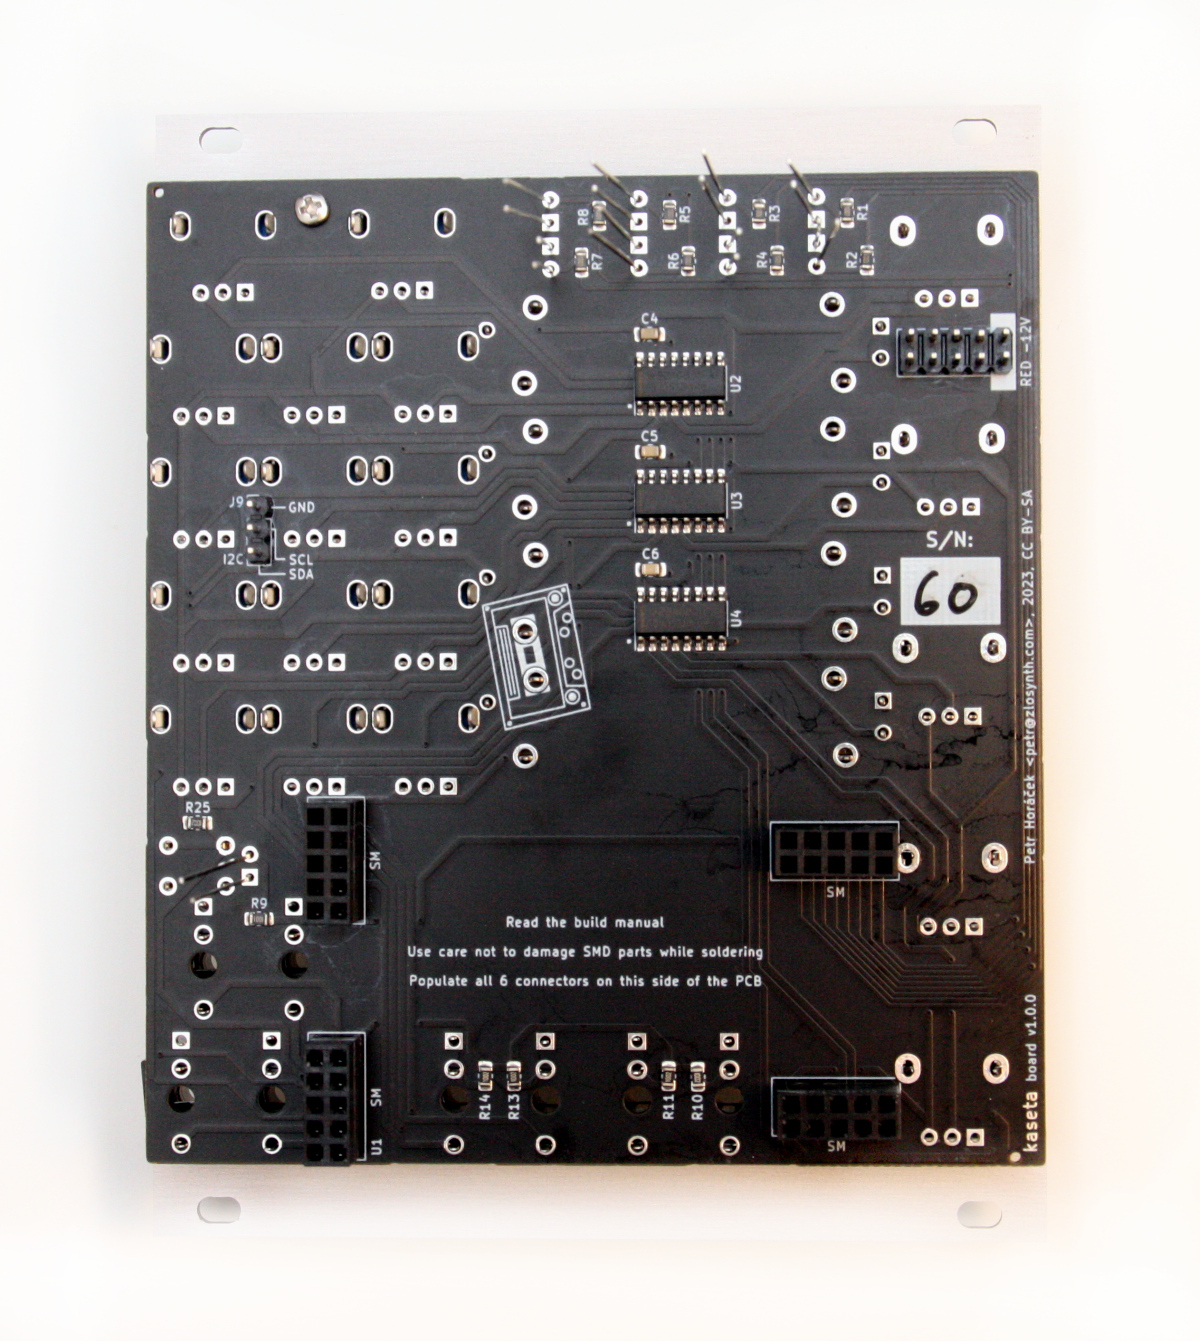
\includegraphics[width=\linewidth]{p04.jpg}
  \caption{Side view with the front components in}
  \label{front components}
\end{figure}

\begin{figure}[p]
  \centering
  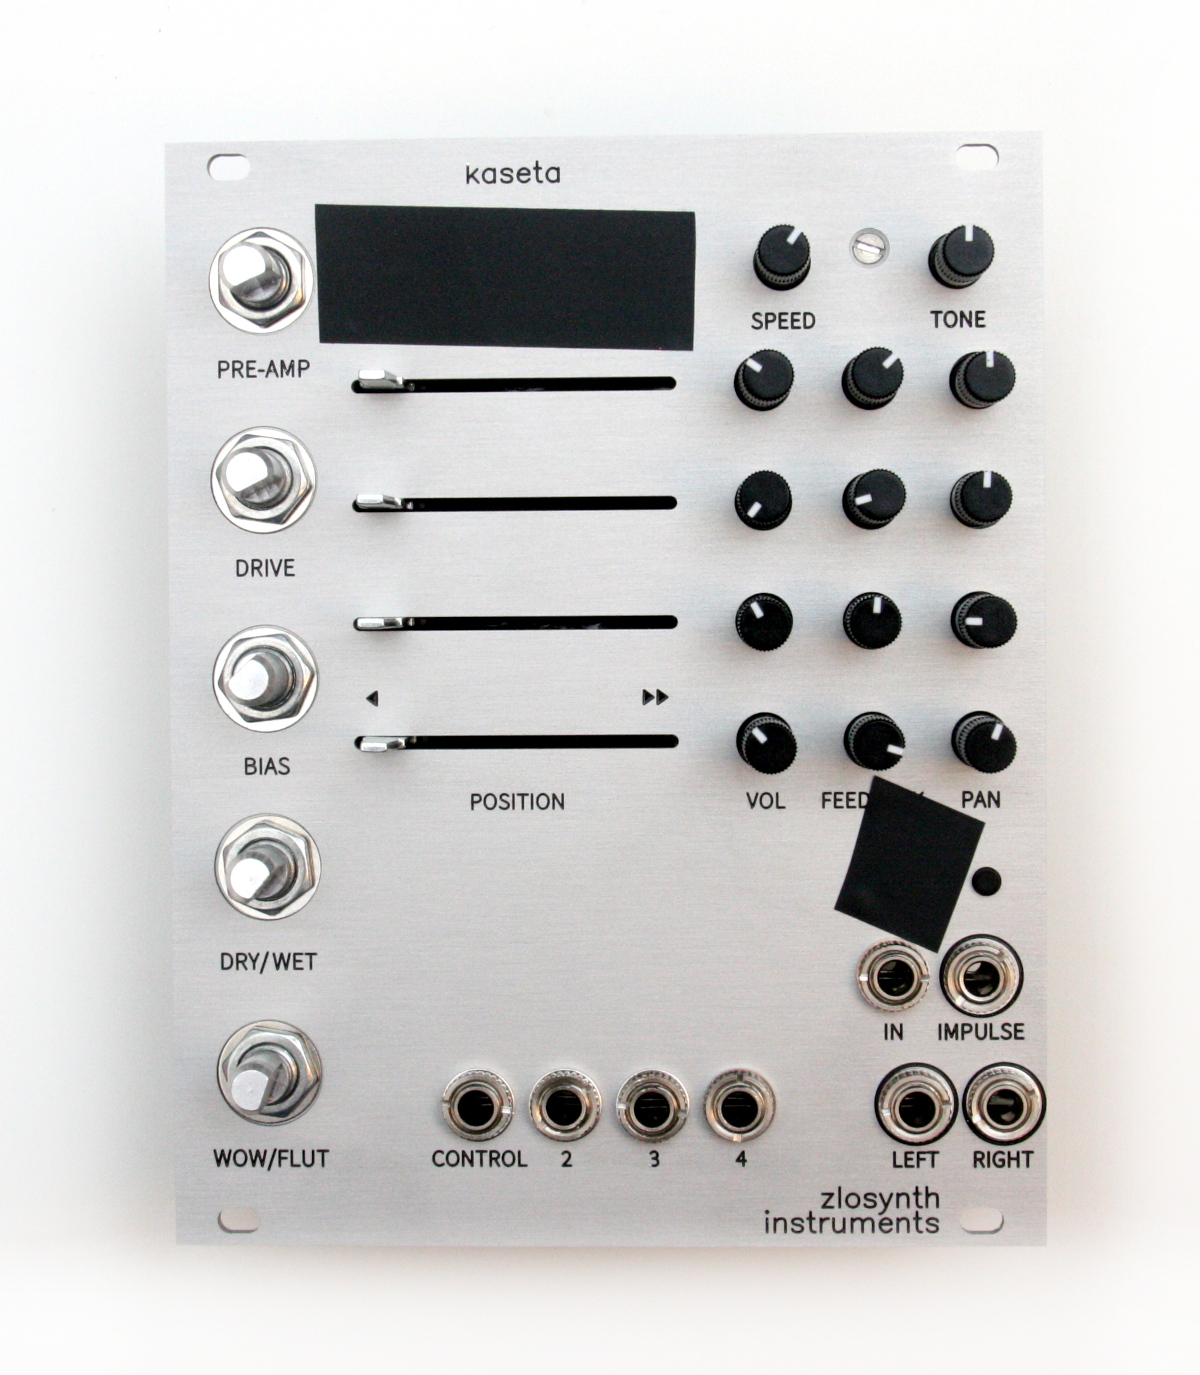
\includegraphics[width=\linewidth]{p05.jpg}
  \caption{Pots and jacks with their washers on}
  \label{washers}
\end{figure}

\begin{figure}[p]
  \centering
  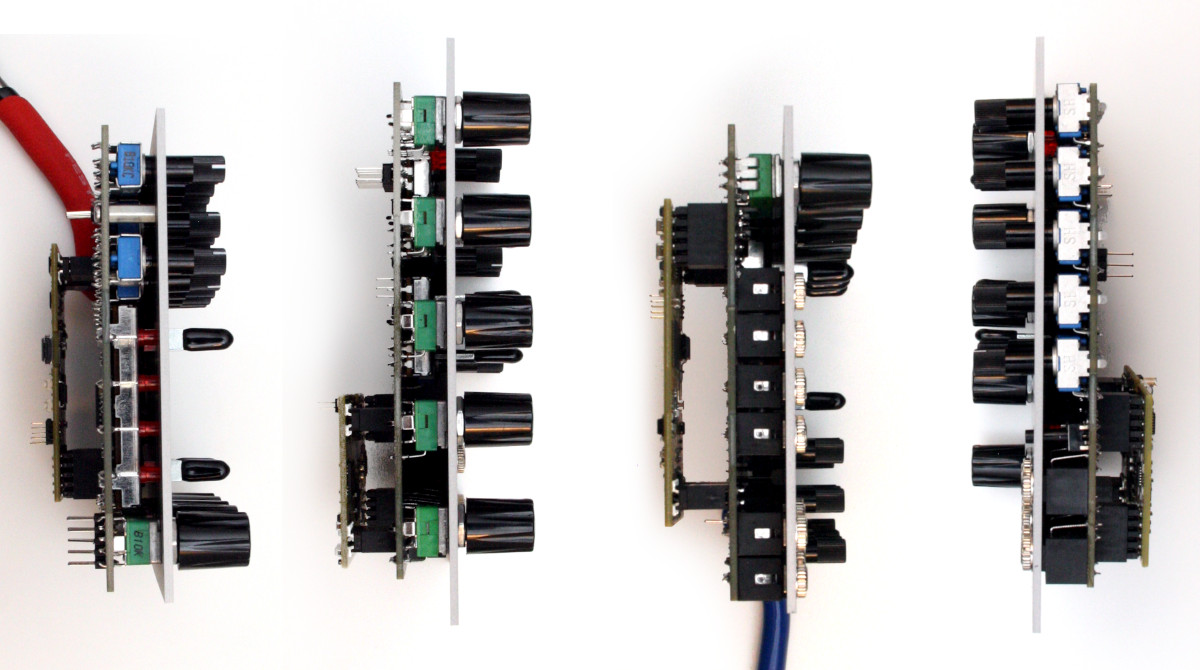
\includegraphics[width=\linewidth]{p06.jpg}
  \caption{Taped LED holes}
  \label{masking}
\end{figure}

% \clearpage

\section{Knobs}

You can now put knobs on the potentiometers.

\begin{enumerate}
  \item The silver part of the big knob is protected with a sticky foil. Peel it off.
  \item Put the big knob on the topmost potentiometer. Use a small flat screwdriver to tighten the screw of the pot. The screw should be pressing against the flat part of the shaft. Keep some distance between the knob and the panel.
  \item Put smaller black knobs on the remaining pots. Align them with the D-shaped shaft and press them in. You may need to pull them a little bit if you see they are scratching the nut.
\end{enumerate}

\begin{figure}[p]
  \centering
  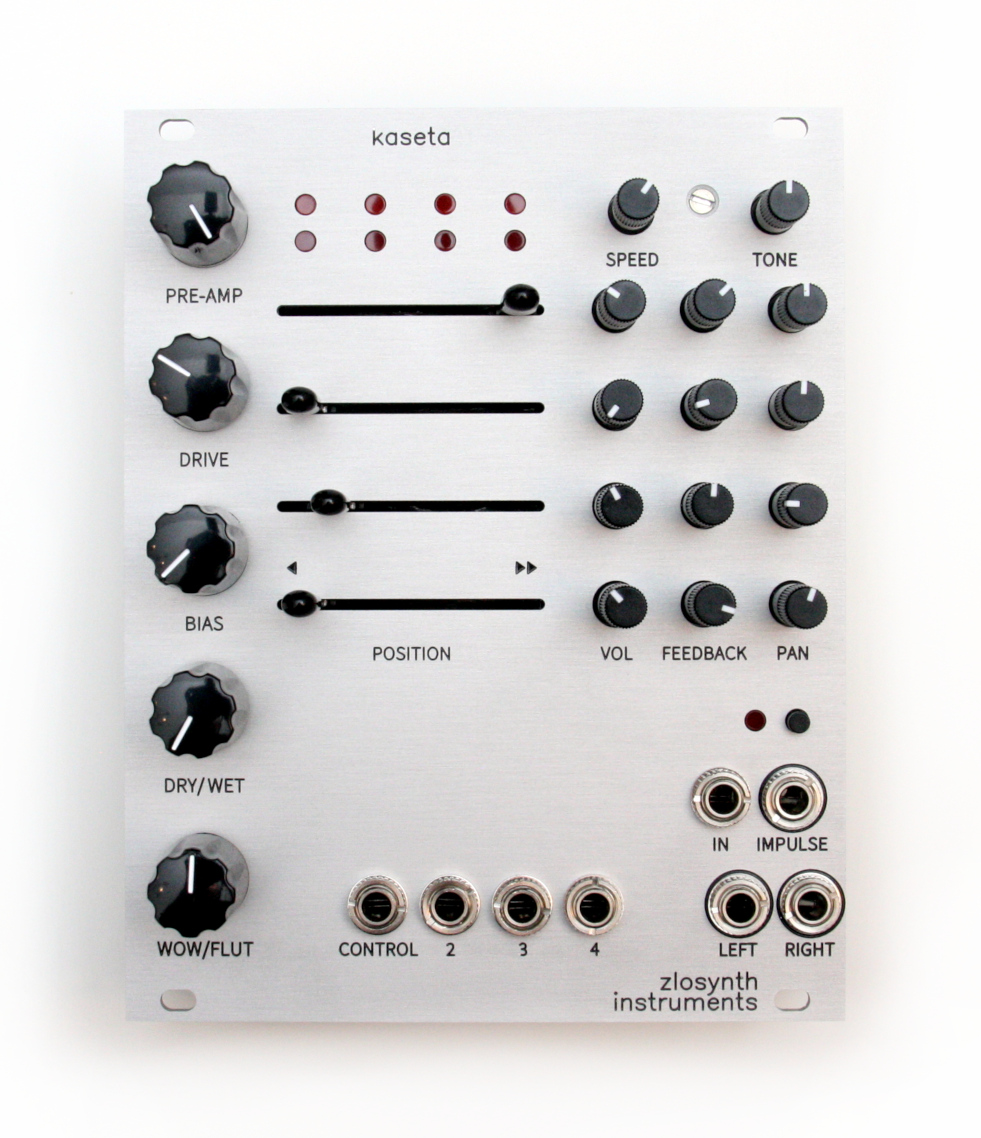
\includegraphics[width=\linewidth]{p07.jpg}
  \caption{Side view of the assembled module}
\end{figure}

\section{Final assembly}

Connect the Daisy Patch Submodule to the main black PCB to complete the build.

\begin{figure}[p]
  \centering
  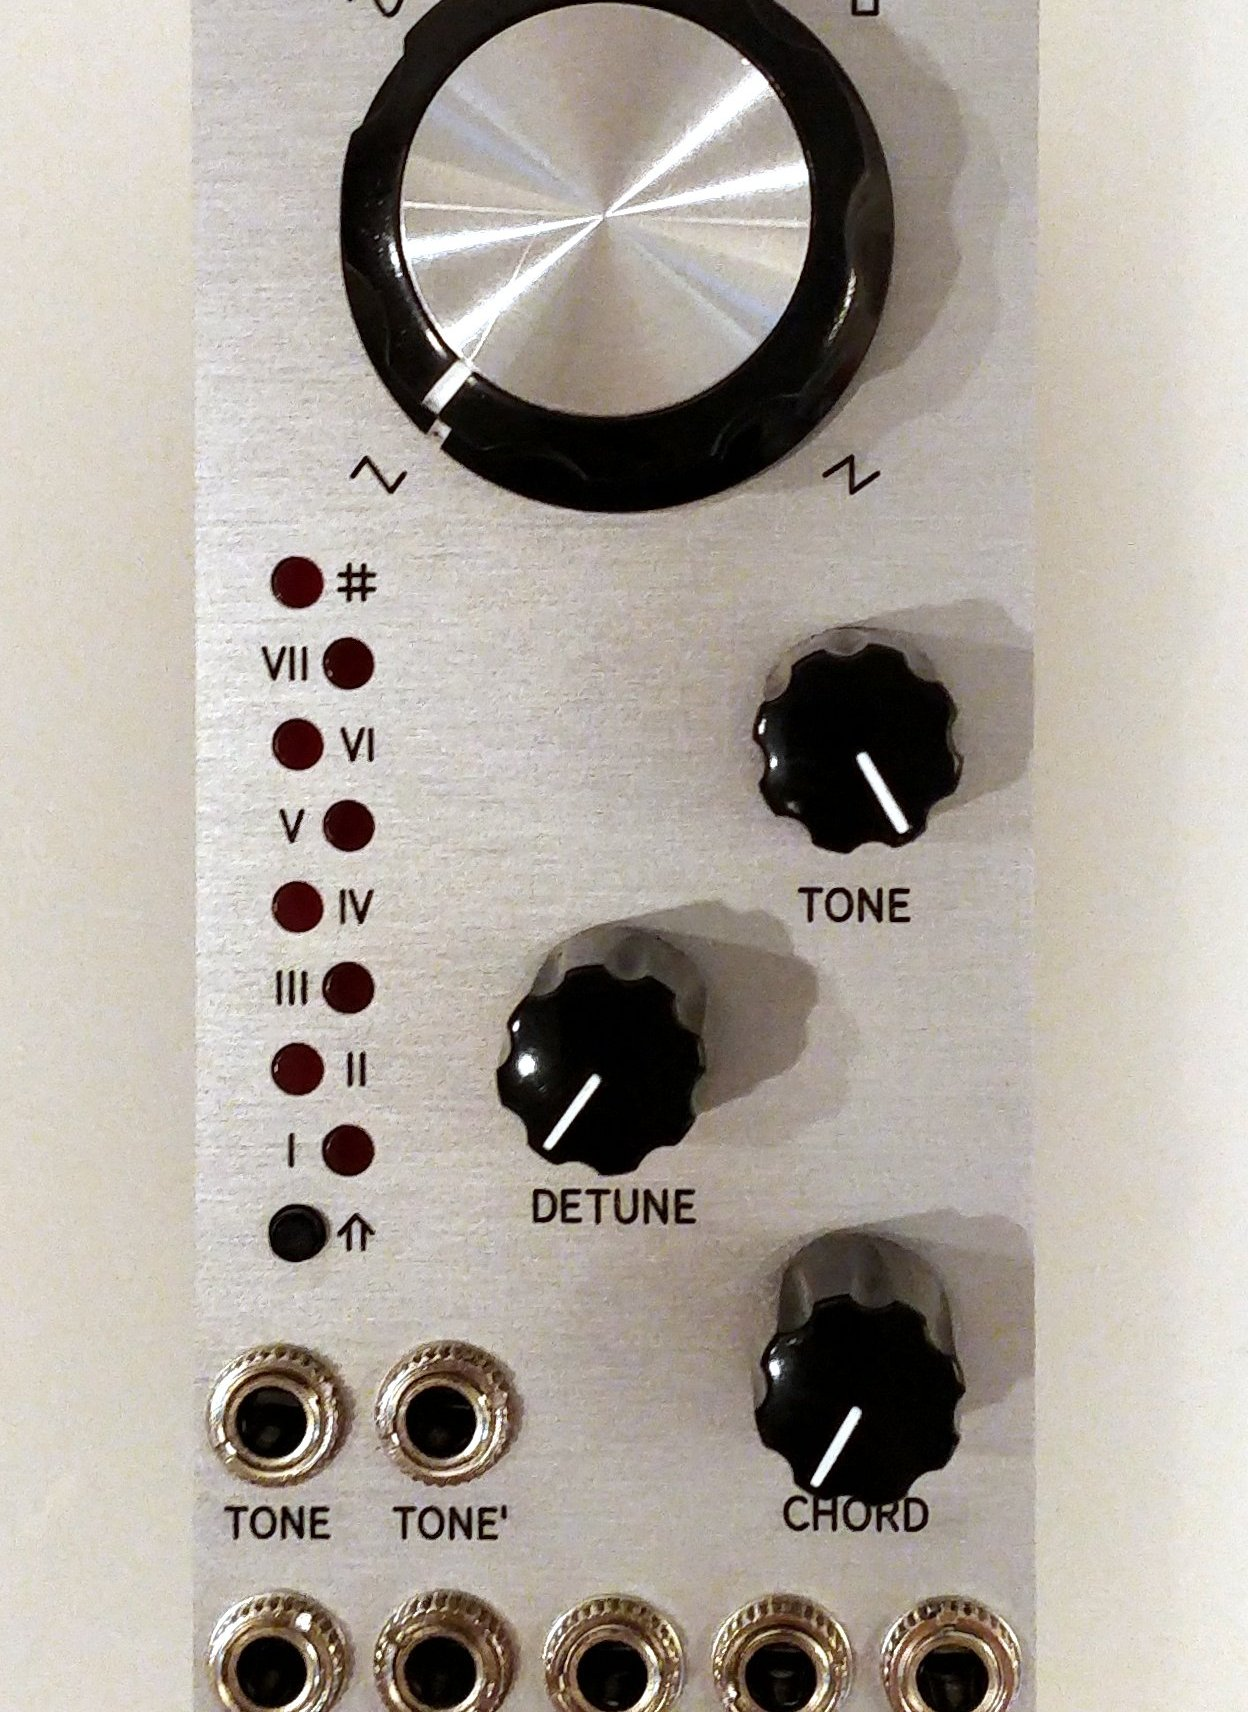
\includegraphics[width=\linewidth]{p08.jpg}
  \caption{Front view of the assembled module}
\end{figure}

\section{Congratulations}

The module is now complete. Have fun!

You can find the user manual on \url{https://zlosynth.com/kaseta-user-manual.pdf}.

\end{document}
